%%%%%%%%%%%%%%%%%%%%%
%								%
%	ESTADO DEL ARTE				%
%								%
%%%%%%%%%%%%%%%%%%%%%
\chapter{Estado del Arte}\label{cap:estadoArte}

%Por definición \textit{e-Commerce}: Transacción comercial electrónica, así como sobre Internet.
%
%Vender y realizar transacciones como estas se pueden hacer gracias a \textit{World Wide Web}, el cual es una convinación global de \textit{links}, información, paginas \textit{web} y \textit{e-Commerce websites}.
%
%Con el fin de considerar 

%TODO


\textit{Open-source e-Commerce shopping carts} ofrecen muchas ventajas para \textit{small businesses}. Soluciones \textit{Open-source} pueden ser desarrolladas para ajustarse a las necesidades del negociante. Ellos contienen una gran combinación de características a un mínimo costo. Y, aunque las opciones de soporte pueden ser mas limitadas que las propietarias o \textit{hosted platforms}, soluciones independientes \textit{open-source} generalmente tienen grandes comunidades de desarrolladores y socios para ayudar a los nuevos comerciantes.

Aquí hay una lista de 11 \textit{open-source e-Commerce solutions}. El \textit{core} de todas las aplicaciones es \textit{free}. Cada aplicación tiene extensiones \textit{free} y \textit{premium} y opciones de soporte para mejorar el desarrollo de la \textit{store}.

\newcommand{\nameOpenCart}{OpenCart }
\subsection{\nameOpenCart}

\begin{figure}[h!]
	\centering
	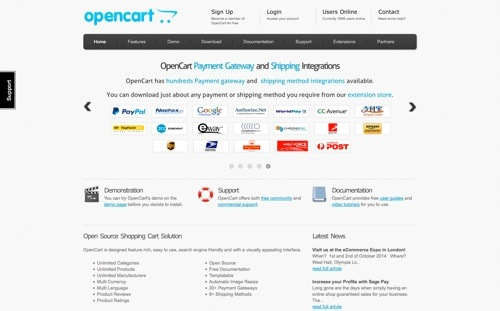
\includegraphics[width=0.5\textwidth]{figuras/cap1/openCartWebsite.jpg}
	\caption{\nameOpenCart \textit{website}\cite{online_OpenCartWebsite}.}
\end{figure}

\nameOpenCart es una aplicación \textit{open-source}, basada en PHP, es una solucion \textit{e-Commerce} para comerciantes \textit{online}. \nameOpenCart tiene una comunidad activa y leal para el apoyo de usuarios, así como una lista de socios comerciales para instalación y customizacion profesional. En \nameOpenCart existen mas de 20 medios de pago, y mas de 8 métodos de envío para la descarga por defecto, con cientos de métodos adicionales para el envío y el pago en su directorio de extensiones. \nameOpenCart también fue diseñado para un manejo sencillo de múltiples compras desde una interfaz de administración. Tiene mas de 2700 \textit{themes}.

\newcommand{\namePrestaShop}{PrestaShop }
\subsection{\namePrestaShop}

\begin{figure}[h!]
	\centering
	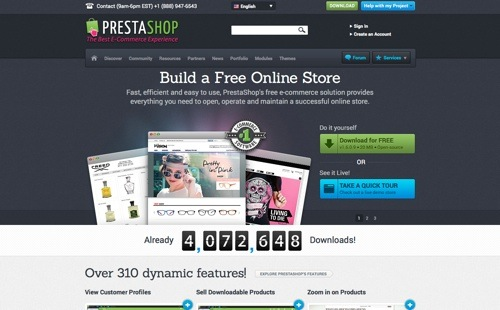
\includegraphics[width=0.5\textwidth]{figuras/cap1/PrestaShopWebsite.jpg}
	\caption{\namePrestaShop \textit{website}\cite{online_PrestaShop}.}
\end{figure}

\namePrestaShop es una solución \textit{e-Commerce} \textit{open-souce}, escrita en PHP y basada en \textit{Smarty template engine}. \namePrestaShop viene con mas de 310 características integradas y 3500 modulos y \textit{templates}. Cuenta con ventas cruzadas, productos descargables, la exportación de productos, una pagina de pago, envio, descuentos y mucho mas. Descargado mas de 4 millones de veces, \namePrestaShop es usado en 160 países y traducido a 63 idiomas. Tiene mas de 600000 miembros en su comunidad.

\newcommand{\nameMagento}{Magento }
\subsection{\nameMagento Community Edition}

\begin{figure}[h!]
	\centering
	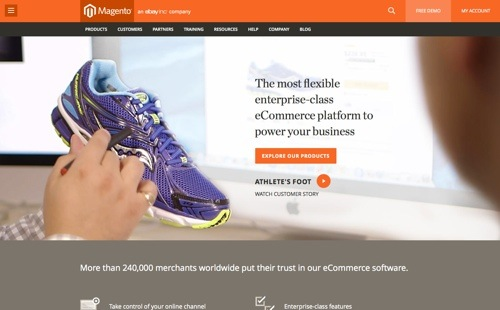
\includegraphics[width=0.5\textwidth]{figuras/cap1/MagentoWebsite.jpg}
	\caption{\nameMagento \textit{website}\cite{online_Magento}.}
\end{figure}

\nameMagento Community Edition es una version \textit{free} y \textit{open-source} de  una plataforma \textit{e-Commerce}. Los comerciantes pueden acceder a caracteristicas adicionales instalando las extensiones desde el gran \textit{\nameMagento Connect marketplace}. No existe soporte para \nameMagento Community Edition, así que las respuestas a las preguntas técnicas deben ser resultas a través del foro de usuarios. Un detalle, \nameMagento ha anunciado el cierro de su \textit{hosted solution}, \nameMagento Go, por ahora no habrían problemas con Community Edition. \nameMagento Community Edition soporta mas de 200000 sitios de clientes .

\newcommand{\nameZenCart}{Zen Cart }
\subsection{\nameZenCart}

\begin{figure}[h!]
	\centering
	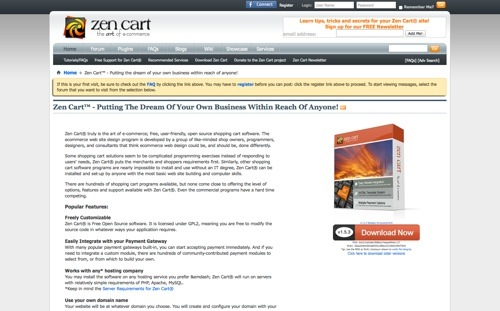
\includegraphics[width=0.5\textwidth]{figuras/cap1/ZenCartWebsite.jpg}
	\caption{\nameZenCart \textit{website}\cite{online_ZenCart}.}
\end{figure}

\nameZenCart es una aplicacion \textit{e-Commerce} \textit{open-source} escrita en PHP.\nameZenCart \textit{branched} desde el código osCommerce en 2003, con una solución que era mas \textit{template-based}. Tiene mas de 1800 \textit{add-ons} en 16 categorias. La comunidad de apoyo de \nameZenCart tiene aproximadamente 150000 miembros y 200000 \textit{threads}.

\newcommand{\nameSpreeCommerce}{Spree Commerce }
\subsection{\nameSpreeCommerce}

\begin{figure}[h!]
	\centering
	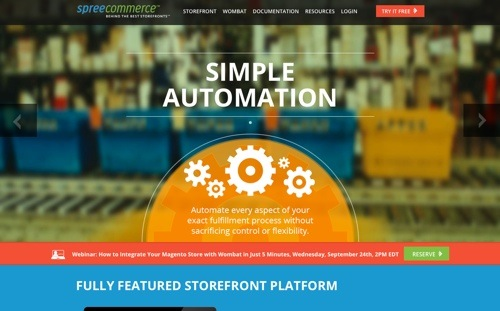
\includegraphics[width=0.5\textwidth]{figuras/cap1/SpreeCommerceWebsite.jpg}
	\caption{\nameSpreeCommerce \textit{website}\cite{online_SpreeCommerce}.}
\end{figure}

\nameSpreeCommerce es una solución \textit{e-Commerce} \textit{open-source}  basado en Ruby on Rails. La plataforma modular permite configurar, complementar, o reemplazar cualquier funcionalidad que necesites. \nameSpreeCommerce tiene mas de 45000 tiendas la plataforma al rededor del mundo, incluyendo Chipotle\cite{online_Chipotle} has more than 45,000 stores using the platform around the world, including Chipotle. Spree Commerce has been translated into more than 30 languages.

\newcommand{\nameDrupalCommerce}{Drupal Commerce }
\subsection{\nameDrupalCommerce}

\begin{figure}[h!]
	\centering
	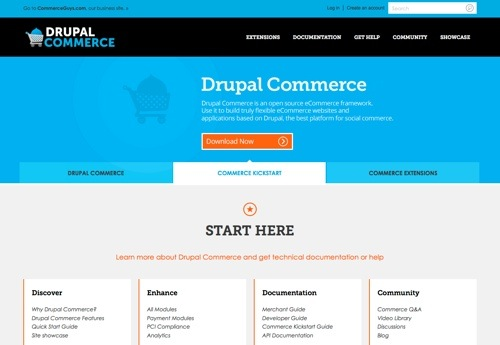
\includegraphics[width=0.5\textwidth]{figuras/cap1/DrupalCommerceWebsite.jpg}
	\caption{\nameDrupalCommerce \textit{website}\cite{online_DrupalCommerce}.}
\end{figure}	

\nameDrupalCommerce es una aplicación \textit{e-Commerce} desarrollado por  Commerce Guys. Construido sobre Drupal content management system. \nameDrupalCommerce ofrece un sistema de administración de producto completo, carro de compra varios lenguajes y monedas; y forma de pago. La lista de extension de \nameDrupalCommerce es una integración completamente en\textit{ third-party} para formas de pago,servicios de cumplimiento, aplicaciones de contabilidad, redes sociales y mucho mas. Paquetes de soporte técnico están disponibles por Commerce Guys.

\newcommand{\nameOsCommerce}{osCommerce }
\subsection{\nameOsCommerce}

\begin{figure}[h!]
	\centering
	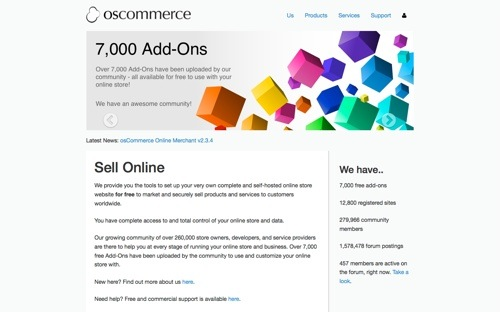
\includegraphics[width=0.5\textwidth]{figuras/cap1/osCommerceWebsite.jpg}
	\caption{\nameOsCommerce \textit{website}\cite{online_osCommerce}.}
\end{figure}

\nameOsCommerce (i.e., \textit{open source Commerce})es uno de las primeras aplicaciones \textit{e-Commerce} \textit{open-source}. Mas de 7000 \textit{free add-ons} han sido subidos por su comunidad para customizar una  \textit{online store}. \nameOsCommerce es usado por cerca de 13000 sitios registrados. La comunidad de apoyo tiene aproximadamente 280000 miembros los cuales han contribuido con 1.5 millones de posts en los foros. La comunidad directa juntos con miembros de otra comunidad están disponibles en vivo en el \textit{Chat room}.

\newcommand{\nameSimpleCart}{simpleCart }
\subsection{\nameSimpleCart}

\begin{figure}[h!]
	\centering
	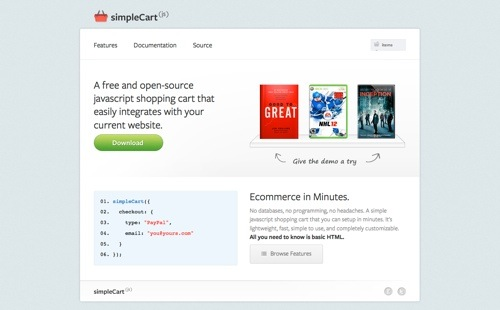
\includegraphics[width=0.5\textwidth]{figuras/cap1/simpleCartWebsite.jpg}
	\caption{\nameSimpleCart \textit{website}\cite{online_simpleCart}.}
\end{figure}

\nameSimpleCart(js) es un \textit{free} y \textit{open-source} JavaScript \textit{shopping cart}. Con su pequeño tamaño, \nameSimpleCart(js) esta disseñado para mantener simple  y sitions con alto trafico \textit{running fast}. \nameSimpleCart(js) tienen la habilidad de pagar con PayPal Express, Google Checkout, y Amazon Payments. \textit{Email checkout} e integracion con  Authorize.Net llegaran pronto.

\newcommand{\nameWooCommerce}{WooCommerce }
\subsection{\nameWooCommerce}

\begin{figure}[h!]
	\centering
	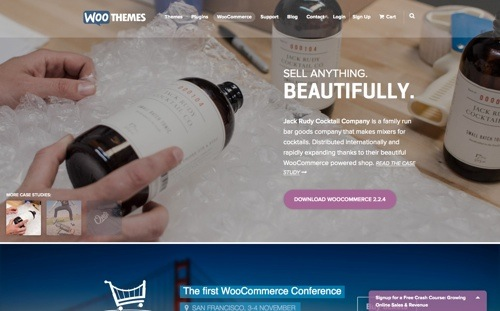
\includegraphics[width=0.5\textwidth]{figuras/cap1/WooCommerceWebsite.jpg}
	\caption{\nameWooCommerce \textit{website}\cite{online_WooCommerce}.}
\end{figure}

\nameWooCommerce es una aplicacion\textit{e-Commerce} \textit{free open-source} que permite a los comerciantes transformar \textit{WordPress sites} en \textit{stores}. \nameWooCommerce fue desarrollado por WooThemes desde un \textit{fork} de Jigoshop. \nameWooCommerce tiene una larga variedad de  \textit{plugins} y  \textit{themes} de WooThemes, como de sitios \textit{third party} tales como ThemeForest\cite{online_ThemeForest} y CodeCanyon\cite{online_CodeCanyon}. Con cerca de 4.5 millones de descargas desde \textit{WordPress.org}\cite{online_WordPress}, \nameWooCommerce es una solucion \textit{e-Commerce} muy popular para WordPress. Para obtener el soporte oficial de WooThemes, es necesario comprar un producto. De otra manera, obtener ayuda desde la comunidad activa del foro.

\newcommand{\nameWPECommerce}{WP e-Commerce }
\subsection{\nameWPECommerce}

\begin{figure}[h!]
	\centering
	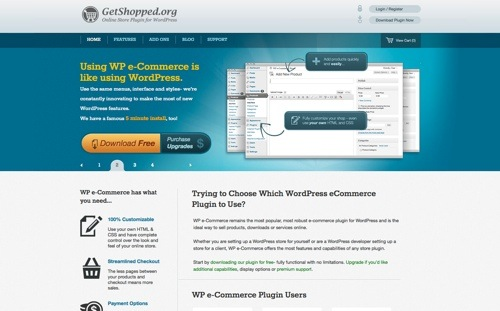
\includegraphics[width=0.5\textwidth]{figuras/cap1/WPECommerceWebsite.jpg}
	\caption{\nameWPECommerce \textit{website}\cite{online_WPECommerce}.}
\end{figure}

\nameWPECommerce es otra aplicacion popular obtenida desde la conversion del  sitio WordPress a una \textit{e-Commerce store}.\nameWPECommerce tiene cerca de 3 millones de descarga de \textit{plugin} desde \textit{WordPress.org}. Usa el propuo HTML y CSS y obten el control completo sobre la vista y la experiencia de tu \textit{online store}.\nameWPECommerce tiene una gran variedad de caracteristicas estandar, incluyendo \textit{ multi-tier pricing} para descuentos por cantidad e integración con redes sociales para \textit{marketing}. Para soporte, hay tutoriales en video y un foro en  \textit{ WordPress.org} ,tambien como consultantes de caracteristicas para ayuda profesional.

\newcommand{\nameJigoshop}{Jigoshop }
\subsection{\nameJigoshop}

\begin{figure}[h!]
	\centering
	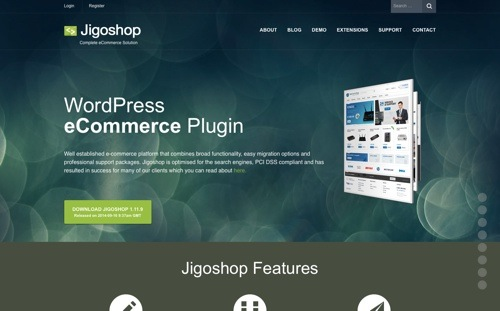
\includegraphics[width=0.5\textwidth]{figuras/cap1/JigoshopWebsite.jpg}
	\caption{\nameJigoshop \textit{website}\cite{online_Jigoshop}.}
\end{figure}

\nameJigoshop es una solucion \textit{e-Commerce} \textit{free} y \textit{open-source} basado en WordPress. Liberado en 2011, \nameJigoshop es el predecesor para WooCommerce. \nameJigoshop tiene mas de 30   \textit{themes}, 100 extensiones, y tres \textit{theme frameworks}. \nameJigoshop es  \textit{free}, asi como el soporte a \textit{WordPress.org}. Sin embago, el acceso a la comunidad de \textit{Jigoshop.com} comienza desde \$40 por mes.



Como se observa, existe una gran cantidad de aplicaciones \textit{open-souce} las cuales están disponibles para ingresar al mundo del comercio electrónico. Todas estas opciones tienen grandes comunidades que las respaldan, asi como muchos usuarios satisfechos. 

Considerando esto, ¿ habrá alguna razón que justifique el desarrollo de un proyecto de estas características?

\section{Justificación para el desarrollo del proyecto}\label{cap:estadoArte:justificacion_proyecto}


\subsection{Base de datos}

base de datos escablaves horizontalmente, SQL escalables verticalmente.




What about transactions?


Many people bring up MongoDB’s lack of atomic transactions across collections as evidence that it’s not suitable for e-commerce applications. This has not been a significant barrier in our experience so far.

There are other ways to approach data integrity. In systems with low-moderate data contention, optimistic locking is sufficient. We’ll share more details about these strategies as things progress.



\begin{table}[h!]
    \tiny
   
%\begin{tabular}{ |C{0.3\paperwidth}|C{0.3\paperwidth}| }
\begin{tabular}{ |l|c|c|c|c| }
\hline
	&
	traider\cite{online_Traider}&
	ReactionCommerce\cite{online_reactionCommerce}&
	NodeShop\cite{online_NodeShop}&
	Forward\cite{online_Forward}
 
\\ \hline
	Tecnología &
	bootstrap, nodejs and mongodb &
	Nodejs, Meteor, Mongodb, CoffeScript, Bootstrap, Docker&
	&
	

\\ \hline
	Mobile &
	&
	&
	&
\\ \hline
	version &
	&
	&
	0.06 ( 21/08/2013 )&
	0.1

\\ \hline
\end{tabular}
    \caption{ Comparación entre diferentes opciones \textit{e-Commerce}}
    \label{tab:wide_table}
\end{table}

\section{Tecnologías }\label{cap:estadoArte:tecnologias}


\subsection{Base de datos}

\textit{Relational databases} se encuentran en la mayoria de las organización desde hace muchisimo tiempo, y por buenas razones. \textit{Relational databases} apoya las aplicaciones del pasado que cumplen con las necesidades de negocio actuales; Estas son apoyadas por un extenso ecosistema herramientas; y hay una gran cantidad de mano de obra calificada para implementar y mantener estos sistemas.
%Relational databases have a long-standing position in most
%organizations, and for good reason. Relational databases
%underpin legacy applications that meet current business
%needs; they are supported by an extensive ecosystem of
%tools; and there is a large pool of labor qualified to
%implement and maintain these systems.

Pero las compañías están cada vez mas considerando la opción de alternativas para la infraestructura relacional heredada. En algunos casos la motivación es técnica, tal como la necesidad de escalar o actuar mas allá de las capacidades de sus sistemas actuales. Mientras que en otros casos, las compañías están motivadas por el deseo de identificar alternativas viables a \textit{softwares} propietario de alto costo. una tercera motivación es la agilidad y velocidad del desarrollo, dado que las compañías ansían adaptarse al mercado mas rápido y adoptar metodologías de desarrollo ágil.
%But companies are increasingly considering alternatives to
%legacy relational infrastructure. In some cases the
%motivation is technical — such as a need to scale or
%perform beyond the capabilities of their existing systems —
%while in other cases companies are driven by the desire to
%identify viable alternatives to expensive proprietary
%software. A third motivation is agility or speed of
%development, as companies look to adapt to the market
%more quickly and embrace agile development
%methodologies.

Estas opciones se aplican tanto para aplicaciones analíticas como transaccionales. Las compañías están cambiando \textit{workloads to Hadoop} para sus \textit{offline}, \textit{analytical workloads}, y están construyendo \textit{online}, aplicaciones operaciones con una nueva clase de tecnología de manejo de datos llamada "\gloss{nosql}", como por ejemplo \textit{MongoDB}
%These drivers apply both to analytical and transactional
%applications. Companies are shifting workloads to Hadoop
%for their offline, analytical workloads, and they are building
%online, operational applications with a new class of data
%management technologies called "NoSQL", or "Not Only
%SQL", such as MongoDB

\subsection{\gloss{sql} and the Relational Model}

\gloss{sql} es un lenguaje declarativo de consulta de datos . Un lenguaje declarativo es uno en el cual un programador specifica lo que desea y el sistema lo ejecuta, en lugar de definir proceduralmente como el sistema deberia hacerlo. Unos pocos ejemplos incluyen: encontrar el registro del empleado 39, mostrar solo el nombre y el numero de telefono del empleado de la totalidad de su registro, filtrar los registros de los empleados a aquellos que trabajan en contabilidad, contar la cantidad de empleados en cada departamento, unir la información de la tabla de los empleados \textit{employees} con la tabla de \textit{managers}.
%SQL is a declarative language for querying data. A declarative language is one in which a programmer specifies what they want the system to do, rather than procedurally defining how the system should do it. A few examples include: find the record for employee 39, project out only the employee name and phone number from their entire record, filter employee records to those that work in accounting, count the employees in each department, or join the data from the employees table with the managers table.


En una primera aproximación, \gloss{sql} permite consultar sobre aquellas preguntas sin pensar sobre como la información es expuesta en el disco, cuales indices utilizar para acceder a la información o que algoritmo utilizar para procesar la información. Un componente arquitectural significativo para la mayoría de los \textit{relational databases is a query optimizer}, el cual decide cual de las muchos equivalentes logicos planea ejecutar las respuesta mas rapida a una \textit{query}. Estos optimizadores son usualmente mejores que los promedios de los usuarios de la \textit{database}, pero en algunas ocasiones ellos no tienen la suficiente información o tienen un modelo muy simple del sistema en \textit{order} para generar ejecuciones mas eficientes.
%To a first approximation, SQL allows you to ask these questions without thinking about how the data is laid out on disk, which indices to use to access the data, or what algorithms to use to process the data. A significant architectural component of most relational databases is a query optimizer, which decides which of the many logically equivalent query plans to execute to most quickly answer a query. These optimizers are often better than the average database user, but sometimes they do not have enough information or have too simple a model of the system in order to generate the most efficient execution.

\textit{Relational databases}, las \textit{databases} mas utilizadas en la practica, siguen el modelo de datos relacional. En este modelo, diferentes entidades del \textit{real-world} son guardadas en diferentes tablas. Por ejemplo, todos los \textit{employees} podrían ser guardados en una tabla \textit{Employees}, y todos los \textit{departments} podrían ser almacenados en la tabla \textit{Departments}.Cada fila de una tabla tiene varias propiedades guardadas en columnas. Por ejemplo, \textit{employees} podrían tener un \textit{employee id}, \textit{salary}, \textit{birth date}, y \textit{first/last names}. Cada una de estas propiedades sera guardada en una columna de la tabla \textit{Employees}
%Relational databases, which are the most common databases used in practice, follow the relational data model. In this model, different real-world entities are stored in different tables. For example, all employees might be stored in an Employees table, and all departments might be stored in a Departments table. Each row of a table has various properties stored in columns. For example, employees might have an employee id, salary, birth date, and first/last names. Each of these properties will be stored in a column of the Employees table.


El modelo relacional, va mano a mano con \gloss{sql}. \textit{Queries} simples de \gloss{sql}, tales como filtrar, recuperar todos los registros el cual sus campos hagan \textit{match} en algunos test( ejemplo, \textit{employeeid} = 3, o salary \> \$ 20000). Constructres mas complejos causan que \textit{database} haga trabajo extra, tal como \textit{joining} información sobre multiples tablas (ejemplo., ¿ Cuál es el nombre del departamento en donde \textit{employee} 3 trabaja?). Otras estructuras complejas tal como \textit{aggregates} (ejemplo, ¿ cuál es el salario promedio de mis empleados?) puede manejar para \textit{full-table scans}.
%The relational model goes hand-in-hand with SQL. Simple SQL queries, such as filters, retrieve all records whose field matches some test (e.g., employeeid
% = 3, or salary \> \$ 20000). More complex constructs cause the database to do some extra work, such as joining data from multiple tables (e.g., what is the name of the department in which employee 3 works?). Other complex constructs such as aggregates (e.g., what is the average salary of my employees?) can lead to full-table scans.


\textit{Relational data model} define entidades altamente estructuradas con relaciones estrictas entre ellos. \textit{Quetying} este modelo con \gloss{sql} permite \textit{complex data transversa} sin desarrollar mucho. La complejidad del modelo y \textit{quering}, tienen sus limites, aunque:
%The relational data model defines highly structured entities with strict relationships between them. Querying this model with SQL allows complex data traversals without too much custom development. The complexity of such modeling and querying has its limits, though:

\textit{Complexity} guia a \textit{unpredictability}. La expresivilidad en \gloss{sql} implica un desafío en relación al costo de cada \textit{query}, y así el costo de \textit{workload}. Mientras, lenguajes de \textit{query} simples pueden complicar la lógica, al mismo tiempo hacen que sea sencillo proveer de almacenamiento de datos., cuando solo responde a \textit{requests} simples.
%Complexity leads to unpredictability. SQL's expressiveness makes it challenging to reason about the cost of each query, and thus the cost of a workload. While simpler query languages might complicate application logic, they make it easier to provision data storage systems, which only respond to simple requests.

Hay muchas maneras modelar un problema. \textit{Relational data model} es estricto: El \textit{schema} asignado para cada tabla especificada la \textit{data} en cada fila. Si se esta almacenando menos \textit{data} estructurada, o filas con mas diferencia en las columnas que se guardan, \textit{relational model} puede ser innecesariamente restrictiva. Similarmente, aplicaciones desarrolladas podrian no encontrar el \textit{relational model} idoneo para modelar cada tipo de \textit{data}. Por ejemplo, una gran cantidad den aplicaciones logicas son escritas en lenguaje \textit{object-oriented} e incluye conceptos \textit{high-level} tales como \textit{lists}, \textit{queues}, y \textit{sets}, y algunos programadores desearan \textit{persistence layer} para modelar esto.
%There are many ways to model a problem. The relational data model is strict: the schema assigned to each table specifies the data in each row. If we are storing less structured data, or rows with more variance in the columns they store, the relational model may be needlessly restrictive. Similarly, application developers might not find the relational model perfect for modeling every kind of data. For example, a lot of application logic is written in object-oriented languages and includes high-level concepts such as lists, queues, and sets, and some programmers would like their persistence layer to model this.

Si la \textit{data} crece mas allá de la capacidad de un servidor, entonces las tablas en la \textit{database} tendrá que ser particionado a través de varios computadores. Para evitar \textit{JOINs} a traves de la red para obtener todas las tablas requeridas, será necesario desnormalizarla. Desnormalizar guarda toda la \textit{data} de diferentes tablas que se desea observar en el mismo lugar. Esto hace que la \textit{database} simule una \textit{key-lookup store system}, dejando preguntas sobre la posibilidad de adaptarse mejor a la \textit{data}.
%If the data grows past the capacity of one server, then the tables in the database will have to be partitioned across computers. To avoid JOINs having to cross the network in order to get data in different tables, we will have to denormalize it. Denormalization stores all of the data from different tables that one might want to look up at once in a single place. This makes our database look like a key-lookup storage system, leaving us wondering what other data models might better suit the data.

Generalmente no es inteligente descartar años de consideraciones de diseño arbitrariamente.Cuando se considera el almacenamiento de la \textit{data} en una \textit{database}, considera \gloss{sql} y \textit{relational model}, los cuales son respaldados por décadas  de investigación y desarrollo, ofreciendo enriquecidas capacidades de modelamiento, y proveer garantías \textit{facil-de-entender} sobre operaciones complejas. \gloss{nosql} es una buena opción cuando se tiene un problema especifico, tal como gran cantidad de \textit{data}, un masivo \textit{workload}, o una difícil desicion de modelamiento para la cual \gloss{sql} y \textit{relational databases} podrían no haber sido optimizadas.
%It's generally not wise to discard many years of design considerations arbitrarily. When you consider storing your data in a database, consider SQL and the relational model, which are backed by decades of research and development, offer rich modeling capabilities, and provide easy-to-understand guarantees about complex operations. NoSQL is a good option when you have a specific problem, such as large amounts of data, a massive workload, or a difficult data modeling decision for which SQL and relational databases might not have been optimized.

\subsubsection{NoSQL}

\gloss{nosql} engloba una gran variedad de diferentes \textit{database technologies} y fueron desarrolladas en respuesta al creciente volumen de \textit{data} guardada de los usuarios, objetos y productos, la frecuencia en que la \textit{data} es accesada, y la \textit{performance} en las necesidades de los procesos. \textit{Relational database}, por otra parte, no fueron diseñadas para hacer frente a los desafíos de escalabilidad y agilidad que enfrentan las aplicaciones modernas, no fueron construidas para tomar ventaja del almacenamiento barato y poder de procesamiento disponible en la actualidad.
%NoSQL encompasses a wide variety of different database technologies and were developed in response to a rise in the volume of data stored about users, objects and products, the frequency in which this data is accessed, and performance and processing needs. Relational databases, on the other hand, were not designed to cope with the scale and agility challenges that face modern applications, nor were they built to take advantage of the cheap storage and processing power available today.

\subsubsection*{Document Model}\label{cap:estadoArte:tecnologias:nosql:document_model}
 Mientras \textit{relational databases store data} en filas y columnas, \textit{document databases store data} en documentos.  

Estos documentos tipicamente usas una estructura equivalente a \gloss{json}, un formato muy popular entre desarrolladores. Documentos proveen una manera intuitiva y natural para modelar \textit{data} que esta cercanamente alineada con  programación \textit{object-oriented}, en el cual cada documento es efectivamente un objeto. Los documentos contienen uno o mas campos, donde cada campo contiene un tipo de valor, tales como \textit{string}, \textit{date}, \textit{binary}, o \textit{array}. En lugar de extenderse un registro entre múltiples tablas y columnas, cada registro y su \textit{data} asociada son tipicamente almacenadas juntas en un solo documento. Esto simplifica el acceso a la \textit{data} y reduce e incluso elimina la necesidad de \textit{joins} y\textit{complex transactions}.

En un \textit{document database}, la nocion de esquema es dinámica: cada documento puede contener diferentes campos. Esta flexibilidad puede ser particulamente util para modelar \textit{data} sin estructura y \textit{polymorphic}. Esto también hace posible la evolución de una aplicación durante su desarrollo, simplemente agregando nuevos campos. Adicionalmente, \textit{document databases} generalmente proveen consultas robustas que los desarrolladores esperan en \textit{relational databases}.

Aplicaciones:\textit{Document databases} son de propósito general y útiles para una amplia variedad de aplicaciones, debido a su flexibilidad del \textit{data model}, la habilidad para consultar sobre cualquier campo y el \textit{natural mapping} del \textit{document data model} a objetos en programación de lenguajes modernos.

Ejemplos: MongoDB y CouchDB.

\subsubsection*{Graph Model}

Basado en \nameref{ap:apendice_B}, usa estructuras de grafos con nodos, bordes y propiedades para representar la \textit{data}. -en esencia, la \textit{data} es modelada como una red de relaciones entre elementos específicos. Si bien es cierto, \textit{Model Graph}, puede ser contra intuitivo y tomar tiempo para entenderlo, puede ser utilizado extensamente para numerosas aplicaciones. Su principal característica es que modela fácilmente las relaciones entre entidades en una aplicación.

Aplicaciones:\textit{Graph databases} son útiles en escenarios donde las relaciones son el \textit{core} de la aplicación, como redes sociales.
Ejemplos: Neo4j y HyperGraphDB.

\subsubsection*{Key-Value}

Desde una perspectiva de\textit{data model}, \textit{key-value stores} son el tipo mas básico de las \textit{\gloss{nosql} databases}. Cada \textit{item} en la \textit{database} es guardado como un atributo \textit{name}, ó \textit{key}, junto con su \textit{value}. El \textit{value}, sin embargo, es totalmente \textit{opaque} al sistema;la \textit{data} solo puede ser requerida desde la \textit{key}. Este modelo puede ser útil para \textit{representig polymorphic} y \textit{unstructured data}, dado que la \textit{database} no define un \textit{scheme} al conjuto \textit{key-value}.
%From a data model perspective, key-value stores are the most basic type of NoSQL database. Every item in the database is stored as an attribute name, or key, together with its value. The value, however, is entirely opaque to the system; data can only be queried by the key. This model can be useful for representing polymorphic and unstructured data, as the database does not enforce a set schema across key-value pairs.

\subsubsection*{Wide Column Models}

Wide column stores, or column family stores, use a sparse,
distributed multi-dimensional sorted map to store data. Each record can vary in the number of columns that are stored, and columns can be nested inside other columns called super columns. Columns can be grouped together for access in column families, or columns can be spread across multiple column families. Data is retrieved by primary key per column family.

Applications: Key value stores and wide column stores are useful for a narrow set of applications that only query data by a single key value. The appeal of these systems is their performance and scalability, which can be highly optimized due to the simplicity of the data access patterns.

2Examples: Riak and Redis (Key-Value); HBase and Cassandra (Wide Column).





\begin{table}[h!]
    \tiny
   
%\begin{tabular}{ |C{0.3\paperwidth}|C{0.3\paperwidth}| }
\begin{tabular}{ |L{0.1\paperwidth}|L{0.3\paperwidth}|L{0.3\paperwidth}|}
\hline
	&
	SQL Databases &
	NoSQL Databases
 
\\ \hline
	Types&
	One type (SQL database) with minor variations&
	Many different types including key-value stores, document databases, wide-column stores, and graph databases
	
\\ \hline
	Development History&
	Developed in 1970s to deal with first wave of data storage applications&
	Developed in 2000s to deal with limitations of SQL databases, particularly concerning scale, replication and unstructured data storage
	
\\ \hline
	Examples&
	MySQL, Postgres, Oracle Database&
	MongoDB, Cassandra, HBase, Neo4j
\\ \hline
	Data Storage Model&
	Individual records (e.g., "employees") are stored as rows in tables, with each column storing a specific piece of data about that record (e.g., "manager," "date hired," etc.), much like a spreadsheet. Separate data types are stored in separate tables, and then joined together when more complex queries are executed. For example, "offices" might be stored in one table, and "employees" in another. When a user wants to find the work address of an employee, the database engine joins the "employee" and "office" tables together to get all the information necessary.&
	Varies based on database type. For example, key-value stores function similarly to SQL databases, but have only two columns ("key" and "value"), with more complex information sometimes stored within the "value" columns. Document databases do away with the table-and-row model altogether, storing all relevant data together in single "document" in JSON, XML, or another format, which can nest values hierarchically.
	

\\ \hline
	Schemas&
	Structure and data types are fixed in advance. To store information about a new data item, the entire database must be altered, during which time the database must be taken offline.&
	Typically dynamic. Records can add new information on the fly, and unlike SQL table rows, dissimilar data can be stored together as necessary. For some databases (e.g., wide-column stores), it is somewhat more challenging to add new fields dynamically.

\\ \hline
	Scaling&
	Vertically, meaning a single server must be made increasingly powerful in order to deal with increased demand. It is possible to spread SQL databases over many servers, but significant additional engineering is generally required.&
	Horizontally, meaning that to add capacity, a database administrator can simply add more commodity servers or cloud instances. The database automatically spreads data across servers as necessary.
	
\\ \hline
	Development Model&
	Mix of open-source (e.g., Postgres, MySQL) and closed source (e.g., Oracle Database)&
	Open-source
	
\\ \hline
	Supports Transactions&
	Yes, updates can be configured to complete entirely or not at all&
	In certain circumstances and at certain levels (e.g., document level vs. database level)
	
\\ \hline
	Data Manipulation&
	Specific language using Select, Insert, and Update statements, e.g. SELECT fields FROM table WHERE…&
	Through object-oriented APIs

\\ \hline
	Consistency&
	Can be configured for strong consistency&
	Depends on product. Some provide strong consistency (e.g., MongoDB) whereas others offer eventual consistency (e.g., Cassandra)

\\ \hline
\end{tabular}
    \caption{ Resumen NoSQL vs. SQL}
    \label{tab:SQL_vs_noSQL_summary}
\end{table}


	\subsection{MongoDB}
	MongoDB (from "humongous") is an open-source document database, and the leading NoSQL database. Written in C++ \cite{technology_mongodb}.
	
	\subsection{Angularjs}
	\cite{technology_angularjs}
	
	\subsection{Bootstrap}
	Bootstrap is the most popular HTML, CSS, and JS framework for developing responsive, mobile first projects on the web \cite{technology_bootstrap}.
	
	\subsection{Nodejs}
	Node.js® is a platform built on Chrome's JavaScript runtime for easily building fast, scalable network applications. Node.js uses an event-driven, non-blocking I/O model that makes it lightweight and efficient, perfect for data-intensive real-time applications that run across distributed devices \cite{technology_nodejs}.
	
	\subsection{CoffeeScript}
	CoffeeScript is a little language that compiles into JavaScript. Underneath that awkward Java-esque patina, JavaScript has always had a gorgeous heart. CoffeeScript is an attempt to expose the good parts of JavaScript in a simple way.
	
	The golden rule of CoffeeScript is: "It's just JavaScript". The code compiles one-to-one into the equivalent JS, and there is no interpretation at runtime. You can use any existing JavaScript library seamlessly from CoffeeScript (and vice-versa). The compiled output is readable and pretty-printed, will work in every JavaScript runtime, and tends to run as fast or faster than the equivalent handwritten JavaScript \cite{technology_coffeescript}.
	
	\subsection{Grunt} 
	\cite{technology_gruntjs}
	
	\subsection{Docker}
	Docker is an open platform for developers and sysadmins to build, ship, and run distributed applications. Consisting of Docker Engine, a portable, lightweight runtime and packaging tool, and Docker Hub, a cloud service for sharing applications and automating workflows, Docker enables apps to be quickly assembled from components and eliminates the friction between development, QA, and production environments. As a result, IT can ship faster and run the same app, unchanged, on laptops, data center VMs, and any cloud\cite{technology_docker}.
	
	




\begin{table}[h!]
    \tiny
   
%\begin{tabular}{ |C{0.3\paperwidth}|C{0.3\paperwidth}| }
\begin{tabular}{ |L{0.1\paperwidth}|L{0.3\paperwidth}|L{0.3\paperwidth}|}
\hline
	\textit{E-Commerce}&
	SQL Databases &
	NoSQL Databases
 
\\ \hline
	El \textit{schema} de los productos varia&
	\textit{Schema} rigido&
	\textit{Schema} flexible
\\ \hline
	Necesita escalar&
	&
	
\\ \hline
	Transacciones&
	&
	
\\ \hline
\end{tabular}
    \caption{ \gloss{nosql} vs. \gloss{sql} en relación a \textit{\gloss{ecommerce}}}
    \label{tab:SQL_vs_noSQL_summary}
\end{table}


\section{MongoDB y E-Commerce \cite{online_mongodb_ecommerce}}\label{cap:estadoArte:MongoDB_ECommerce}

Demostración de \textit{next-generation data stores} tipicamente giran en torno a \textit{social network}: Twitter, Facebook, Foursquare, etc. Desafortunadamente, tales aplicaciones tienden a tener complejos \textit{data models}. \textit{E-Commerce} por ejemplo, tiene la ventaja de incluir un largo número de patrones familiares para \textit{data modeling}. Ademas no es complicado imaginar como \textit{products, categories, product reviews} y \textit{orders} son típicamente modeladas en \gloss{rdbms}.

\textit{E-Commerce} han sido usualmente un dominio exclusivo de \gloss{rdbms}s, y esto es así por un par de razones. La primera, es que \textit{\gloss{ecommerce} sites} generalmente requieren \textit{transactions}, y \textit{transactions} son una operación básica en \gloss{rdbms}. Lo segundo es que, hasta hace poco, dominios que requieren de un \textit{rich data model} y sofisticadas \textit{queries} ha sido presupuesto que se ajustan mejor en \gloss{rdbms}. En las siguientes secciones se cuestionara la segunda afirmación. 

\subsection{\textit{Catalog Management}}

Si es necesaria información sobre como el \textit{catalog management} se maneja con \textit{relational databases}, es necesario dar una mirada rápida a los \textit{schemas} del popular Magento \textit{e-Commerce framework} \ref{ap:figure:catalog_magento} o OfBiz de Apache \ref{ap:figure:catalog_ofbiz}. Lo que se observa es un conjunto de tablas trabajando a la par para proveer un \textit{schema} flexible sobre un fundamentalmente inflexible estilo de \textit{database system}.

Esto significa que la \textit{data} de cualquier producto se extiende a través de una docena de tablas. Esto incremente la complejidad del código requerido para la persistencia de consultas de productos individuales y hacer una consulta \textit{shell-based} es casi imposible. Simplemente considere escribir un \gloss{sql} JOIN para para reunir el modelo de un producto como esto:

\begin{figure}[h!]
	\centering
	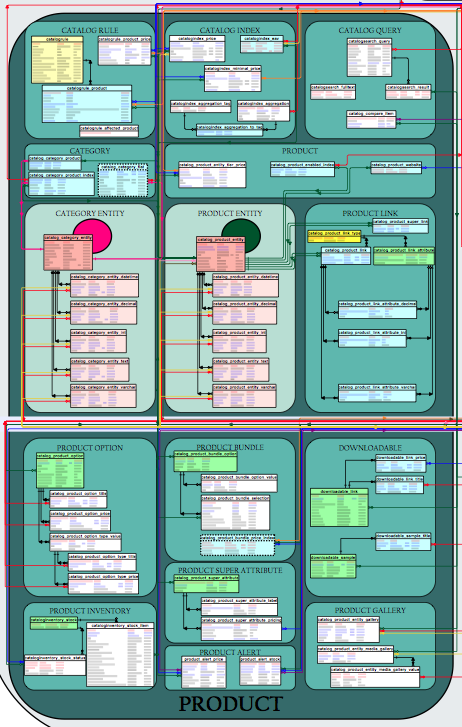
\includegraphics[width=0.3\textwidth]{figuras/cap2/magento_product_schema.png}
	\caption{\textit{Schemas}de un producto.}
	\label{cap:figure:catalog_magento}
\end{figure}

O realizar una sencilla búsqueda desde MongoDB JavaScript \textit{shell} para obtener un objecto \gloss{json} como este:

\medskip
\begin{lstlisting}[caption= Busqueda en MongoDB]

db.products.find({'_id': ObjectID("4bd87bd8277d094c458d2fa5")});

{_id: ObjectID("4bd87bd8277d094c458d2a43"),
 title: "A Love Supreme [Original Recording Reissued]"
 author: "John Coltrane",
 author_id: ObjectID("4bd87bd8277d094c458d2fa5"),

 details: {
   number_of_discs: 1,
   label: "Impulse Records",
   issue_date: "December 9, 1964",
   average_customer_review: 4.95,
   asin: "B0000A118M"
 },

 pricing: {
  list: 1198,
  retail: 1099,
  savings: 99,
  pct_savings: 8
 },

 categories: [
   ObjectID("4bd87bd8277d094c458d2a43"),
   ObjectID("4bd87bd8277d094c458d2b44"),
   ObjectID("4bd87bd8277d094c458d29a1")
 ]
}
\end{lstlisting}

Claramente no es una representación completa de un producto, pero esto demuestra cuantas de estas tablas triviales que existen en una \textit{relational representation} pueden prescindir en un \textit{document representation}.

Para \textit{object-oriented data}, los documentos tienen mayor sentido, tanto en concepto como rendimiento. Una representación \textit{document-oriented} de una \textit{data} de un producto se traduce a unas pocas entidades (un puñado de \textit{collections} vs. una docena de tablas), mejor \textit{performance} en consultas (sin \textit{sever-side joins}), y estructuras que corresponden precisamente al producto. Ya no existe la necesidad de diseñar un \textit{master schema} que pueda considerar a cada tipo de producto concebible.

\textit{Catalog management} es esencialmente \textit{content management}, un campo en donde MongoDB sobresale.

\subsection{Shopping Carts and Orders}

Permitir que un \textit{shopping cart} sea simplemente una orden en un estado del \textit{\"cart\"}, el modelo de \textit{shopping carts} y las ordenes en MongoDB se tornan muy sencillas:

\medskip
\begin{lstlisting}[caption= Estructura de una orden.]

{'_id': objectid('4b980a6dea2c3f4579da141e'),
 'user_id': objectid('4b980a6dea2c3f4579a4f54'),
 'state': 'cart',

 'line_items': [
    {'sku': 'jc-432',
     'name': 'John Coltrane: A Love Supreme',
     'retail_price': 1099
    },

    {'sku': 'ly-211',
     'name': 'Larry Young: Unity',
     'retail_price': 1199
    },
  ],

 'shipping_address': {
   'street': '3333 Greene Ave.',
   'city': 'Brooklyn',
   'state': 'NY',
   'zip': '11216'
  },

  'subtotal': 2199
}
\end{lstlisting}

Notar que es posible presentar los pedidos como un \textit{array} de productos. Como es usual con documentos, esto hace el despliegue del \textit{shopping cart} mas sencillo, dado que no hay \textit{joins} envueltos. Pero esto también resuelve el problema del versionamiento de productos. Usualmente es necesario tener el estado de un producto cuando este es comprado. Esto puede ser logrado en una \gloss{rdbms} estableciendo un vinculo a versiones particulares de un producto. Aquí, sin embargo, simplemente se almaceno el estado de un producto dentro de la misma orden.

\subsection{\textit{Querying Orders}}

Dado que MongoDB soporta consultas dinámicas y \textit{secondary indexes}, las consultas para las ordenes son automáticas. Es posible, por ejemplo, definir un \textit{index} en un \textit{product \gloss{sku}}, lo que permite consultas eficientes en todas las ordenes para un producto dado:

\medskip
\begin{lstlisting}[caption= Consulta eficiente con \textit{secondary indexes}.]
	db.orders.ensureIndex({'line_items.sku': 1});
	db.orders.find({'line_items.sku' => 'jc-431'});
\end{lstlisting}

Con MongoDB, es posible realizar consultas en atributos arbitrarios, de esa manera cualquier \textit{query}, en \textit{orders collection} es posible. Y para \textit{queries} comunes, es posible definir \textit{indexes} para una mejor eficiencia.

\subsection{\textit{Aggregation}}

Claramente, \textit{aggregation} también es necesario. Se desea reportar ordenes de diferentes maneras, y para ese propósito, \textit{map-reduce} esta disponible. Como ejemplo, el comando \textit{map-reduce} que \textit{aggregtes} el total de ordenes por \textit{zip code}:

\begin{lstlisting}[caption= Ejemplo de commando \textit{map-reduce}.]
map = "
  function() {
    emit(this['shipping_address']['zip'], {total: this.total})
  }"

reduce = "
  function(key, values) {
    var sum = 0;
    values.forEach(function(doc) {
      sum += doc.total;
    }

    return {total: sum};
  }"


db.orders.mapReduce(map, reduce, {out: 'order_totals_by_zip'});
\end{lstlisting}

\subsection{Updating Orders}

\subsubsection{Incrementing Quality}

Una manera de ajustar la cantidad es usando un \textit{position operator}, el cual permite aplicar \textit{atomic operations}, a un único objeto dentro de un \textit{array}. A continuación se muestra como cambiar el numero de álbumes que se están ordenando:

\begin{lstlisting}[caption= Ejemplo de \textit{atomic operation}.]
	db.orders.update({'_id': order_id, 'line_items.sku':'jc-431'},
		{'$set': {'line_items.$.quantity': 2}});
\end{lstlisting}

 
\subsubsection{Adding and Removing Items}

Igualmente, \textit{atomic operators} resuelven el problema de agregar y remover productos desde el carro. Por ejemplo, se puede utilizar \$push \textit{atomic operator} para agregar un item al \textit{cart};

\begin{lstlisting}[caption= Ejemplo de \textit{atomic operation}.]
	db.orders.update({'_id': order_id},
    {'$push': {'line_items':
      {'sku': 'md-12', 'price': 2500, 'title': 'Basketball'}}
     '$inc': {'subtotal': 2500}});
\end{lstlisting}

Al ajustar la cantidad y el cambio de los mismos \textit{items} en el \textit{cart}, es necesario actualizar el total de la orden. Notar el uso de \$inc \textit{operator} para manejar esto.

\subsection{Inventory}

No todos los sitios \textit{e-Commerce} necesitan manejar el inventario. Pero para aquellos que si lo hacen, MongoDB funciona a la altura de las circunstancias.

Una manera para manejar el inventario, es \textit{store} un documento separado por cada \textit{physical item} en la bodega. Así, por ejemplo, si la bodega tiene veinte copias del álbum Coltrane, se traduce en veinte documentos distintos en \textit{inventory collection}. Cada documento tiene una estructura como la siguiente:

\begin{lstlisting}[caption= Ejemplo de \textit{atomic operation}.]
	{'_id': objectid('4b980a6dea2c3f4579da432a'),
 'sku': 'jc-431',
 'state': 'available',
 'expires': null,
 'order_id': null
}
\end{lstlisting}


Cuando un usuario intenta agregar un \textit{item} al \textit{cart}, un \textit{findAndModify command} puede ser facilitado para \textit{atomically mark} el \textit{item} en \textit{in-cart}, asociando el \textit{item} con una orden dada, y estableciendo un tiempo de expiración:

\begin{lstlisting}[caption= Ejemplo de \textit{atomic operation}.]
	query = {'sku': 'jc-431', 'state': 'available'};

update = {'$set':
          {'state':    'cart',
           'order_id': order_id,
           'expires':  Date.now() + 15 * 60}};

item = db.inventory.findAndModify(query: query, update: update);
\end{lstlisting}

Si se obtiene un \textit{item back} desde el \textit{findAndModify operation}, se sabe que tenemos un único \textit{lock} en el \textit{item}, y es posible \textit{store it} en el \textit{cart}. Cuando el usuario desea \textit{check out}, el estado del \textit{item} puede cambiar a \textit{"purchased"}, o cualquiera sea el caso de la llamada.

Mientras, se pueda ejecutar un \textit{script in the background} que libere el inventario del \textit{cart} que no ha sido \textit{purchased} en la ventana de quince minutos. La actualización es trivial:

\begin{lstlisting}[caption= Ejemplo de \textit{atomic operation}.]
	db.inventory.update({'state': 'cart', 'expires': {'$lt': Date.now()}},
  {'$set' {'state': 'available', 'expires': null, 'order_id': null}},
  {multi: true});
\end{lstlisting} 

\subsection{\textit{Transactions}, \textit{Consistency} y \textit{Durability}}

Muchos argumentos impuestos contra NoSQL en \textit{e-Commerce} se centran en \textit{transactions}, \textit{consistency}, y \textit{durability}. En relación a esto se mencionan algunos puntos.

En relación a \textit{transactions}, ciertamente MongoDB no soporta el tipo \textit{multi-object}; sin embargo, soporta \textit{atomic operations} sobre documentos individuales. y esto combinado con \textit{documento-oriented modeling} recién descrito y creatividad, es suficiente para muchos problemas \textit{e-Commerce}. Ciertamente, si se necesita \textit{debit one account} y \textit{credit another} en la misma operación, o si se desea \textit{rollback}, sera necesario \textit{full-fledged transactions}. No obstante, \textit{transactionality} provista por MongodB debería ser suficiente en la mayoría de los casos, si no en todos, para \textit{e-Commerce operations}.

Si la preocupación esta sobre \textit{consistency} y \textit{durability}, operaciones escritas en MongoDB pueden ser realizadas \textit{consistency} sobre conexiones. Ademas, MongoDB 1.5 soporta \textit{near-real-time replications}, así que es posible asegurarse que una operación ha sido \textit{replicated} antes de retornar.

\subsection{\textit{Scalability}}
La manera mas sencilla para \textit{scale} la mayoría de las \textit{databases}, es \textit{upgrading} el \textit{hardware}. Si la aplicación esta corriendo en un único nodo, es usualmente posible agregar una combinación de \textit{disk} IOPS, \textit{memory}, y CPU para eliminar los cuello de botella de la \textit{database}.La técnica de mejorar el \textit{hardware} de un solo node para escalar se conoce como \textit{vertical scaling} o \textit{scaling up}. \textit{Vertical scaling} tiene la ventaja de ser simple, seguro, y \textit{cost-effective} hasta un cierto punto. Si se esta ejecutando sobre un \textit{virtualized hardware}( tal como \textit{Amazon's EC2}), entonces puedes encontrar que una instancia lo suficientemente larga no esta disponible. Si estas ejecutando sobre \textit{physical hardware}, habrá un punto donde el costo de un servidor mas poderoso se vuelve prohibitivo.

\begin{figure}[h!]
	\centering
	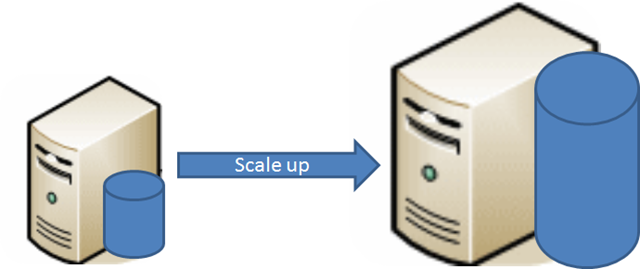
\includegraphics[width=0.5\textwidth]{figuras/cap2/scale_up.png}
	\caption{\textit{Vertical scaling} o \textit{Scaling up} }
\end{figure}

Entonces tiene sentido  considerar \textit{scaling horizontally} o \textit{scaling out}. En lugar de reforzar un único nodo, \textit{scalling horizontally} significa distribuir de \textit{database} sobre múltiples maquinas. Dado que \textit{horizontally scaled architecture} puede utilizar \textit{comodity hardware}, el costo de \textit{hosting} el total de la \textit{data} puede ser reducido significativamente. Incluso, la distribución  de \textit{data} sobre maquinas mitiga las consecuencias de fallo. Las maquinas inevitablemente fallaran de algún momento a otro. Si se \textit{scaled vertically} , y la maquina falla, entonces es necesario tratar con una falla en un maquina de la cual la mayoría del sistema depende. Podría no considerarse un tema si una copia de la \textit{data} existe en un \textit{replicated slave}, pero aun esta el caso e que solo un único \textit{sever} es necesario para bajar el sistema completo. En contraste con el fallo dentro de un \textit{horizontally scaled architecture}. Esto podría ser menos catastrófico dado que una sola máquina representa un porcentaje menor del sistema completo.

\begin{figure}[h!]
	\centering
	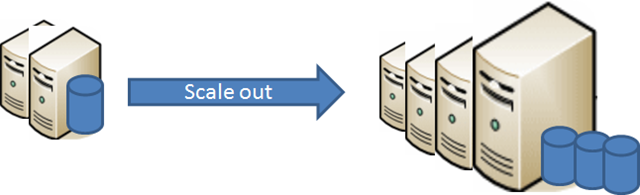
\includegraphics[width=0.5\textwidth]{figuras/cap2/scale_out.png}
	\caption{\textit{Horizontally scaling} o \textit{Scaling out} }
\end{figure}

MongoDB es un \textit{database management system} diseñado para hacer \textit{horizontal scaling} manejable, dado que fue construido para aplicaciones \textit{web} e infraestructuras de Internet.

\subsection{Conclusion}

Es cierto que la mayoría de \textit{NoSQL databases} no fueron construidas considerando \textit{e-Commmerce}. \textit{Databases} que carecen \textit{data models} enriquecidos, \textit{dynamic queries}, y la noción de \textit{transactionality} no puede esperarse que compitan en el espacio de \textit{e-Commerce}, entonces no es comprensible que no se considere MongoDB tampoco.

Pero para las partes en donde el sitio \textit{\gloss{ecommerce}} comprende el manejo de contenido, MongoDB es claro vencedor. E incluso para mas \textit{transactional components} del sistema, MongoDB tiene características que hacen de la posibilidad de correr un sistema completo de \textit{e-Commerce} una realidad.